
\documentclass[a4paper,12p]{article}

% used to specify page dimentions
\usepackage[includeheadfoot,margin=2.5cm]{geometry}

% used to modify the header and the footer
\usepackage{fancyhdr}
\pagestyle{plain}

% used to change font (for this to work you need to change your engine to xelatex or luatex)
\usepackage{fontspec}
\setmainfont{Times New Roman}

% used to change paragraph spacing and line spacing
\usepackage{setspace}
\centering
\setlength{\parskip}{6pt}
\renewcommand{\baselinestretch}{1.5}

% used to set default section and subsection font sizes and spacing and style
\usepackage{titlesec}
\usepackage{sectsty}

\titleformat*{\section}{\fontsize{14pt}{12pt}\bfseries\raggedright}
\titleformat*{\subsection}{\fontsize{12pt}{6pt}\bfseries\raggedright}
\titleformat*{\subsubsection}{\fontsize{10pt}{5pt}\bfseries\raggedright}

% used to set the numbering of sections and subsections
\renewcommand\thesection{\arabic{section}}
\renewcommand\thesubsection{\thesection.\arabic{subsection}}

% used to generate random text, use \lipsum[n] where n is the number of paragraphs
\usepackage{lipsum}

% for lists
\usepackage{enumitem}
\setlist{nosep}

% for images
\usepackage{graphicx}
\graphicspath{{images/}}
\usepackage[figurename=Figure]{caption}
\renewcommand{\figurename}{Figure}

\begin{document}
    % write content here
    % % you will get a compilation error if this section is empty

    % add title

    % add authors
    \begin{center}
        \textbf{Raid Nasrellah TEYAR} \\
        \textbf{Oussama SALAHOUELHADJ} \\
        \textbf{Mohammed Elhadi SAOUDI} \\
    \end{center}

    \raggedright\section{Les besion fonctionnelle et l'identification des cas d'utilisation}


    \subsection{Les besion fonctionnelle}

    \begin{itemize}

        \item{Authentication functional requirements:}
        \begin{itemize}
            \item Login
            \item retrieve password if forgotten
        \end{itemize}

        \item{Modul management functional requirements:}
        \begin{itemize}
            \item Consult modules he is responsible of
        \end{itemize}

        \item{Question bank/module management functional requirements:}
        \begin{itemize}
            \item Create a bank of questions
            \item Import a bank of questions
            \item Consult a bank of questions
            \item Modify a bank of questions
            \item Delete a bank of questions
            \item Export a banks of questions
        \end{itemize}

        \item{Question management functional requirements:}
        \begin{itemize}
            \item Create a question
            \item Import list of questions
            \item Consult a question
            \item Modify a question
            \item Delete a question
            \item Duplicate a question
            \item Export list of questions
            \item Search/sort/filtre questions
        \end{itemize}

        \item{Exam management functional requirements:}
        \begin{itemize}
            \item Create an exam
            \item Import an exam
            \item Consult an exam
            \item Modify an exam
            \item Delete an exam
            \item Export an exam
            \item Search/sort/filter exams
            \item Try an exam
            \item Duplicate an exam
            \item Consult list of response
            \item Confirm evaluation
            \item Consult list of reclamation
            \item Consult exam session
            \item Consult exam analytics
            \item Publish an exam
        \end{itemize}

        \item{Response management functional requirements:}
        \begin{itemize}
            \item Consult a response
            \item Evaluate a response
            \item Export a response
            \item Search/filter/sort responses
        \end{itemize}

        \item{Student management functional requirements:}
        \begin{itemize}
            \item Affect students to an exam
            \item Delete student from an exam
        \end{itemize}

        \item{Modify his own profile}

        \item{Claims management functional requirements:}
        \begin{itemize}
            \item Consult a claim
            \item Mark a claim as done
            \item Report student
            \item Reply to a reclamation
        \end{itemize}

        \item{examsToProcotor management functional requirements:}
        \begin{itemize}
            \item Consult list of exams to proctor
            \item Consult exam to proctor
        \end{itemize}
    \end{itemize}

    \clearpage
    \subsection{DCU de chaque acteur}
    % when using images you just have to include the name of the image without the extension

    \begin{figure}[h]
        \centering
        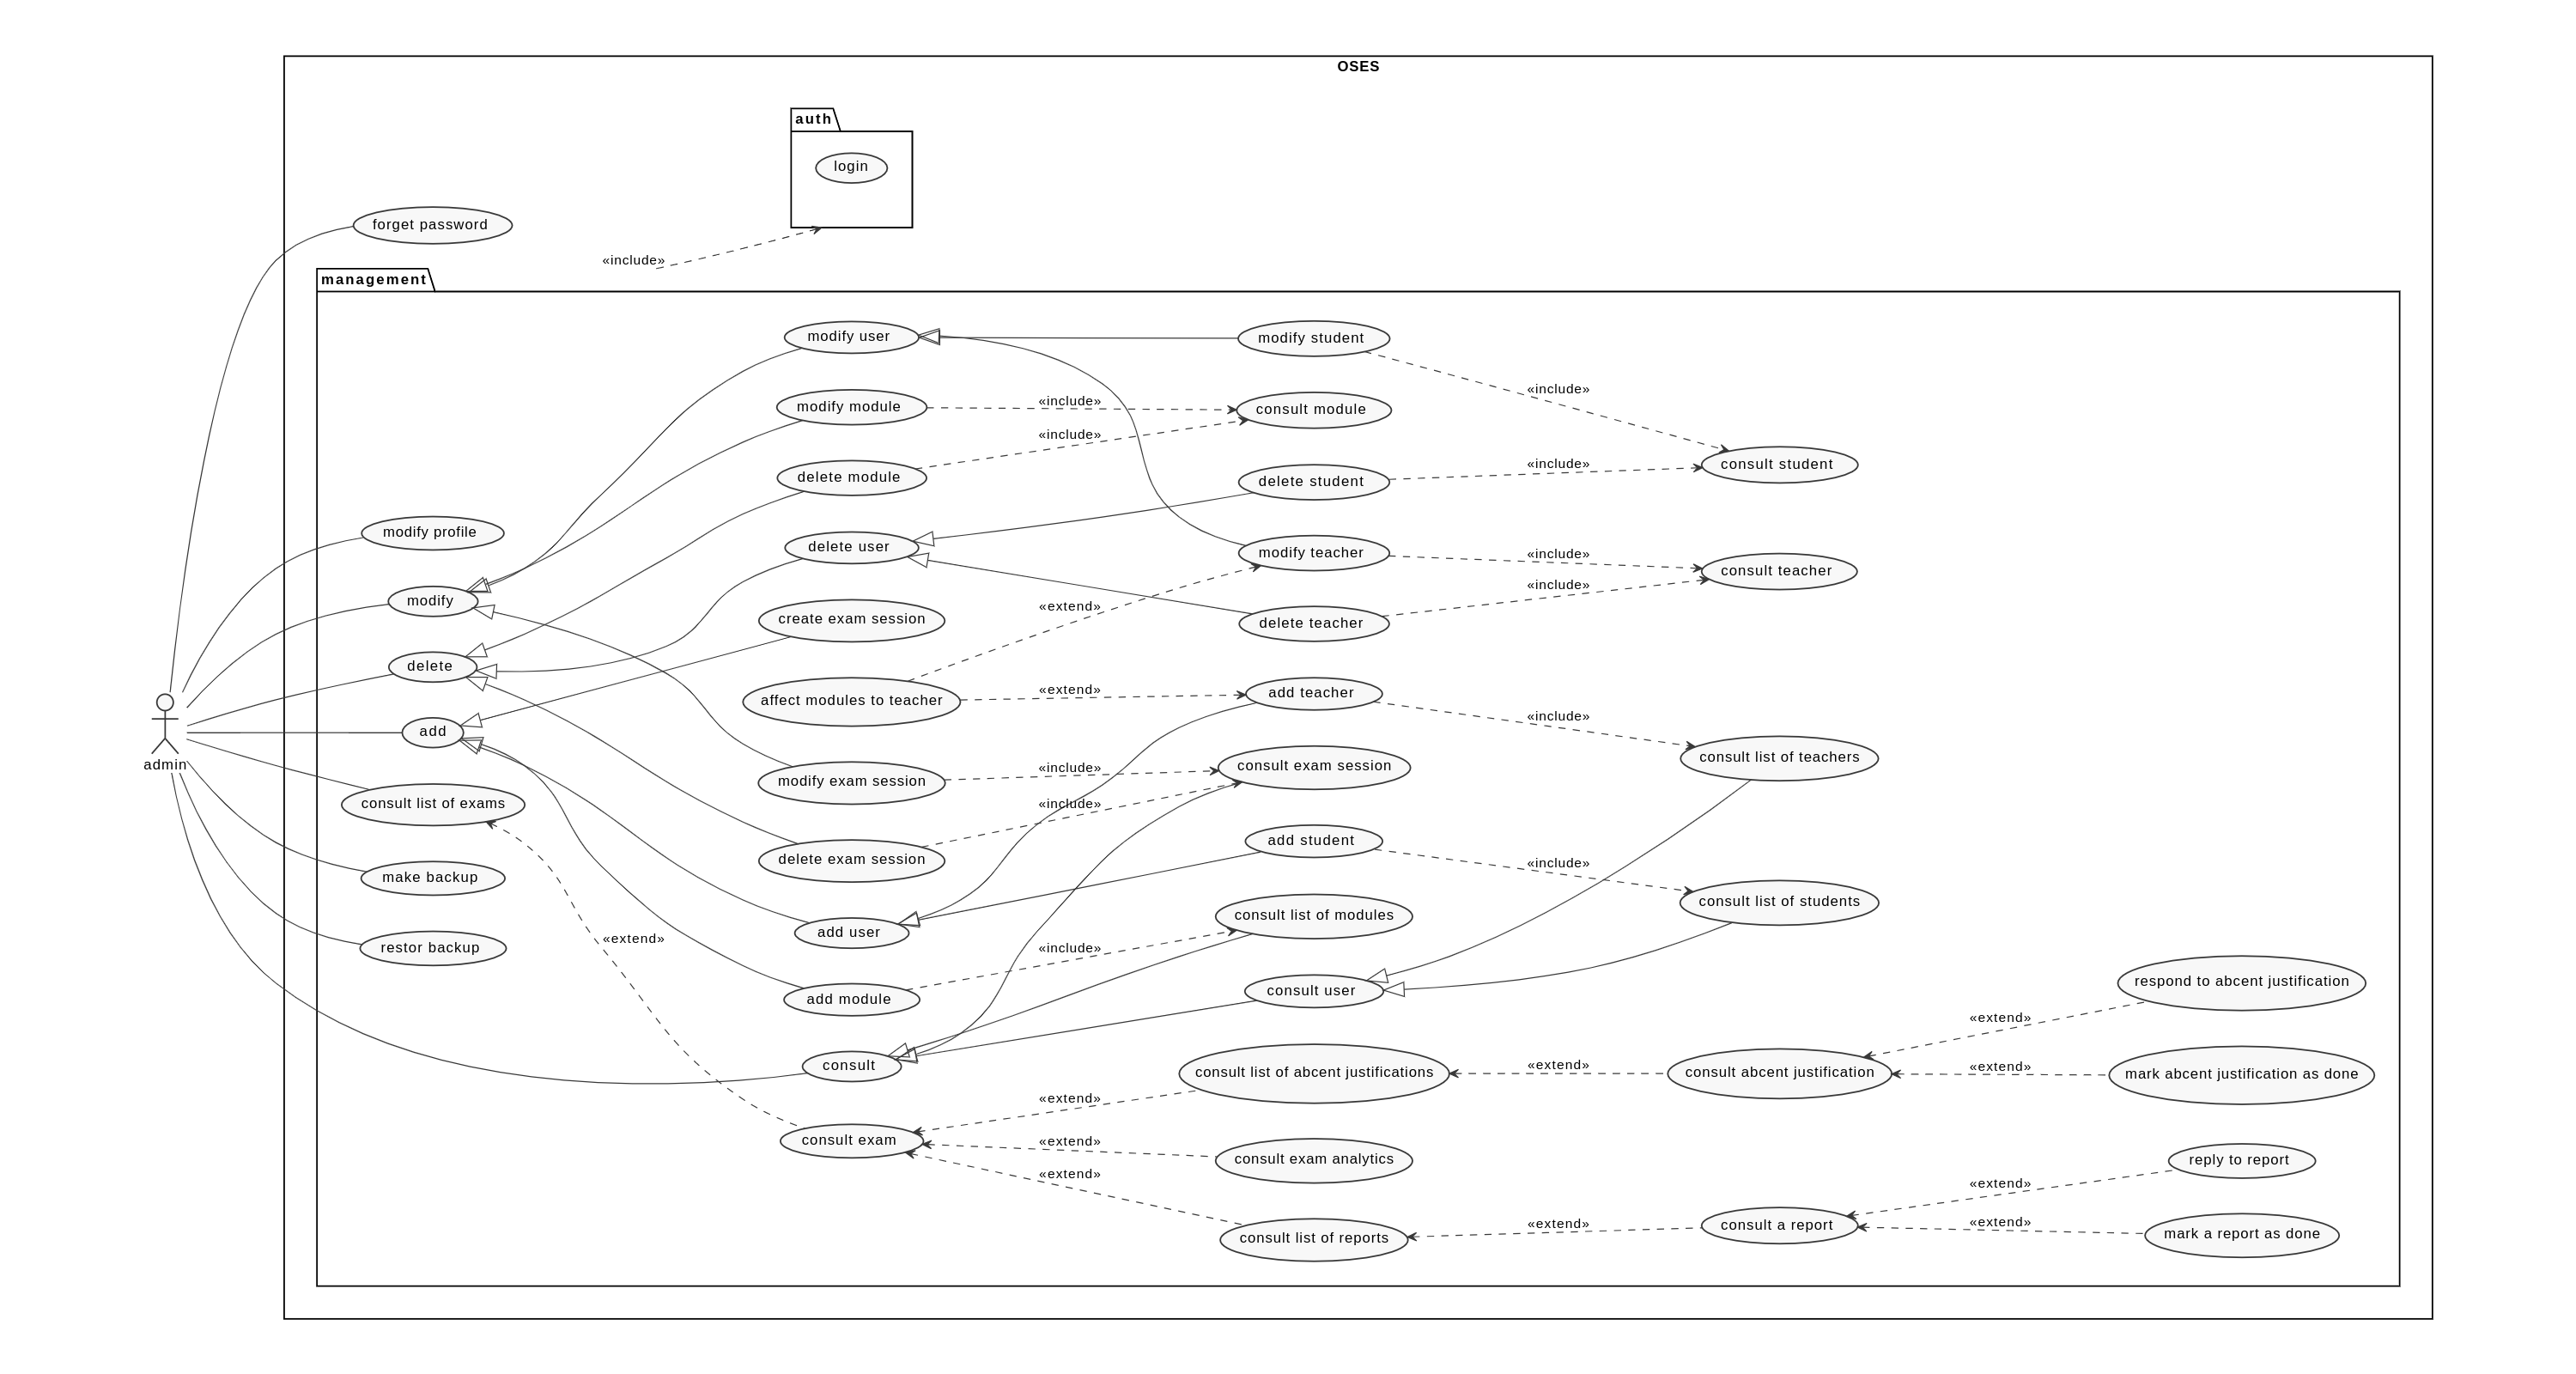
\includegraphics[width=\textwidth]{admin_UCD}
        \caption{admin use case diagram}
    \end{figure}

    \begin{figure}[h]
        \centering
        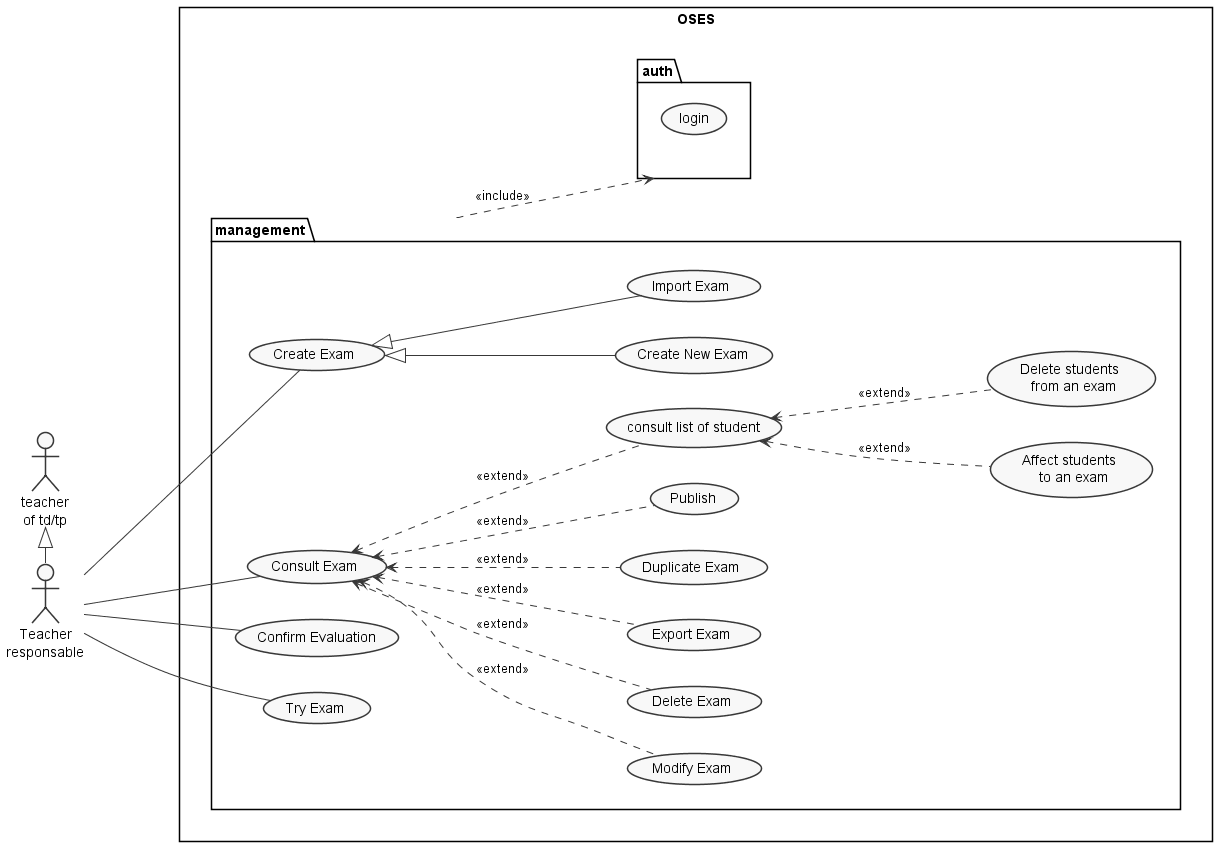
\includegraphics[width=\textwidth]{Module_Teacher}
        \caption{module teacher use case diagram}
    \end{figure}

    \begin{figure}[h]
        \centering
        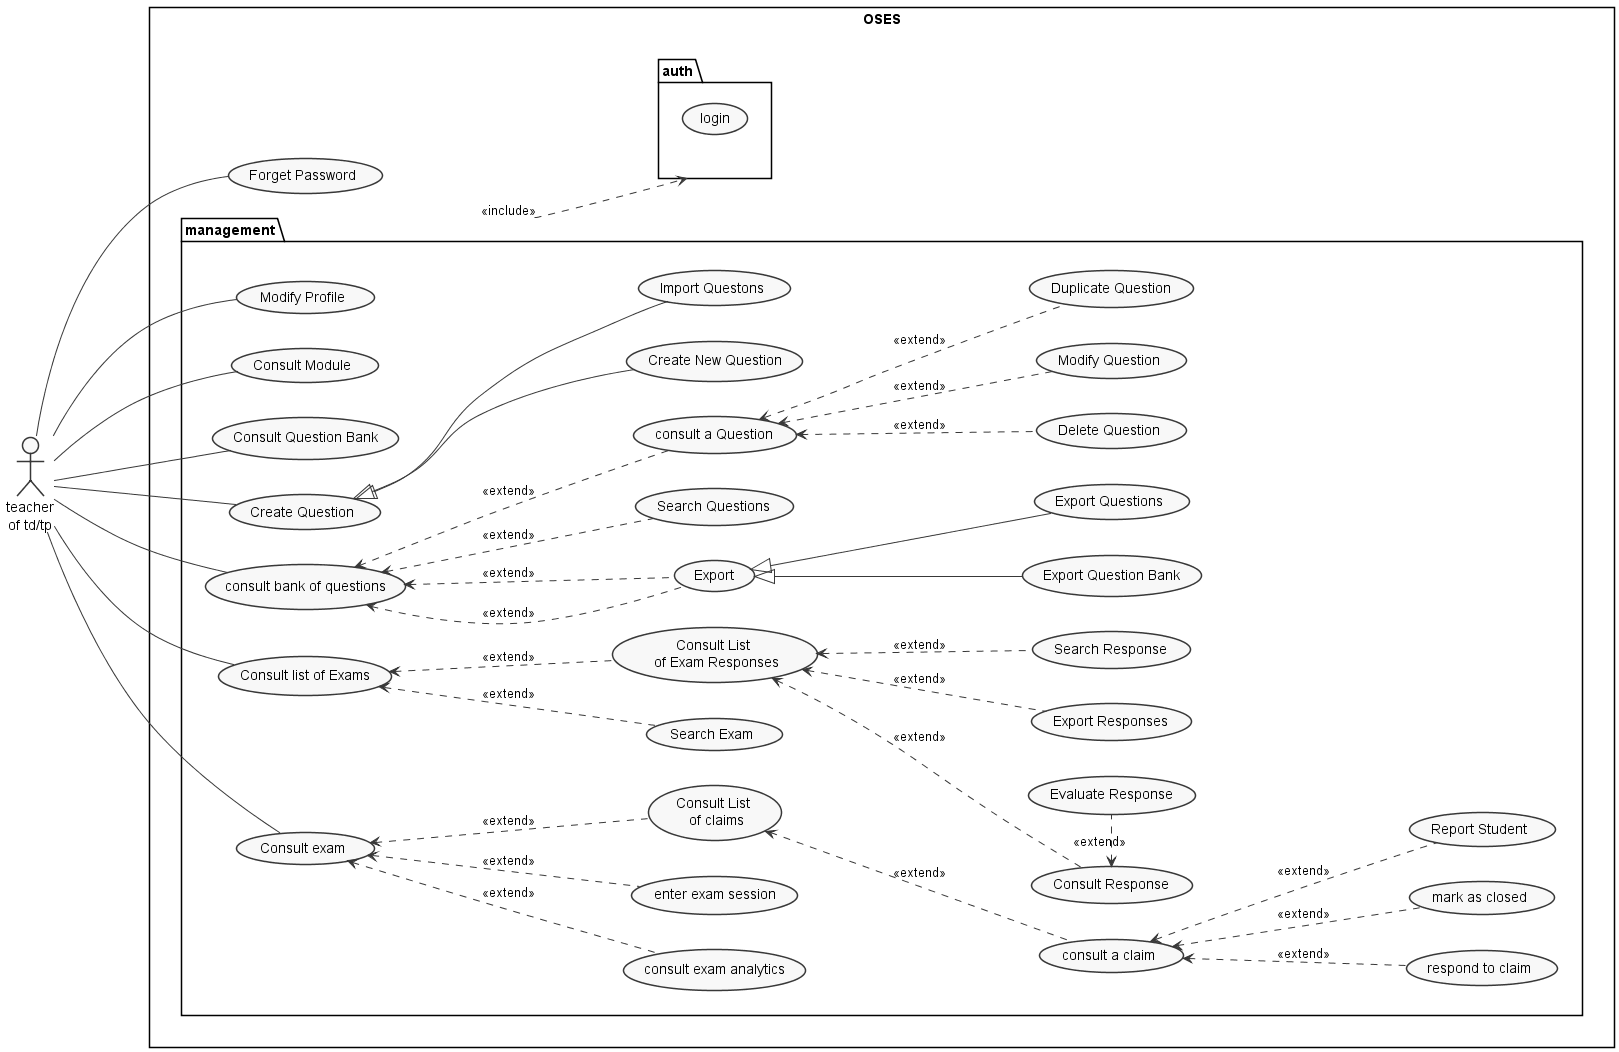
\includegraphics[width=\textwidth]{TP TD_Teacher}
        \caption{Td/Tp teacher use case diagram}
    \end{figure}

    \begin{figure}[h]
        \centering
        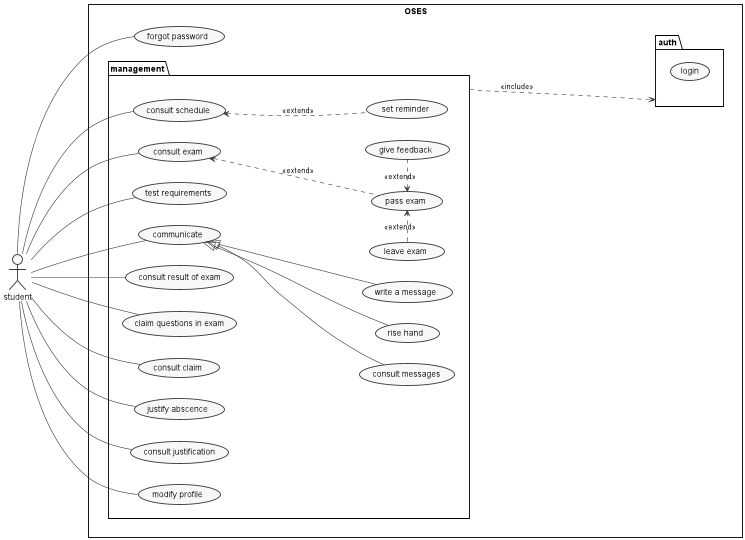
\includegraphics[width=\textwidth]{student_UCD}
        \caption{student use case diagram}
    \end{figure}

    \begin{figure}[h]
        \centering
        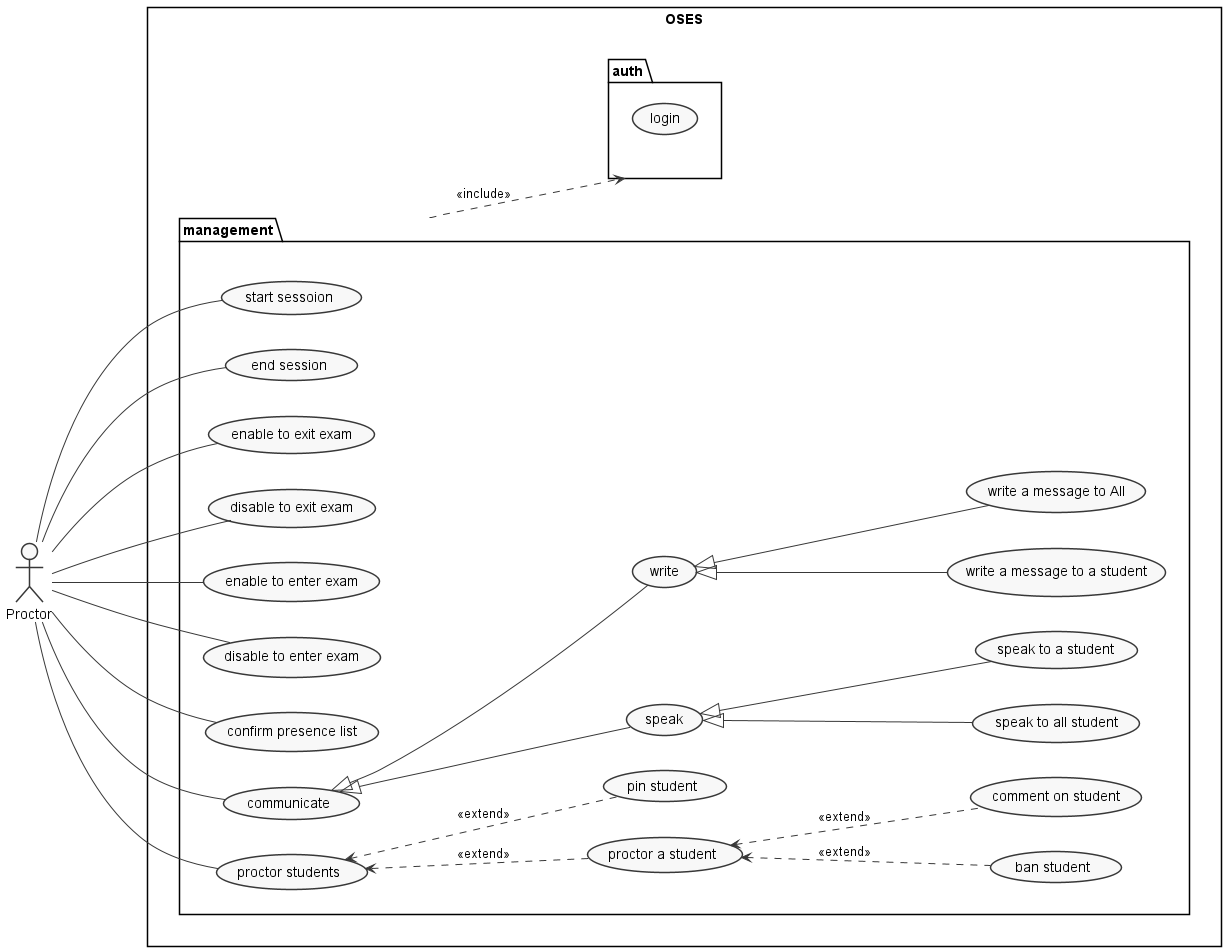
\includegraphics[width=\textwidth]{proctor_UCD}
        \caption{proctor use case diagram}
    \end{figure}

\end{document}